%!TEX root = ../../../_main.tex
\section{Main Thesis}
\label{sec:main-thesis}

\begin{ques}
	\typedlabel{ques:main}
	Let $(W,S)$ be a Coxeter system, $\theta : W \to W$ an automorphism of $W$ with $\theta^2 = \id$ and $\theta(S) = S$, and $K \subset S$ a subset of $S$ generating a finite subgroup of $W$ with $\theta(K) = K$. Futhermore let $T,S_1,S_2,S_3 \subset S$ be four pairwise disjoint sets of generators. For which Coxeter groups $W$ does the implication
	\begin{equation}
		\label{eq:main}
		w \in w_K C_{T \cup S_i}, i=1,2,3 \Rightarrow w \in w_K C_T
	\end{equation}
	hold for any possible $K,\theta,T,S_1,S_2,S_3$ and $w$?
\end{ques}

The reader might wonder, why we handle with three sets $S_1,S_2,S_3$ and not just with two. The reason for that is also the main reason, why $Wk(\theta)$ is less accessible than $\Br(\ti{\theta})$: In $Wk(\theta)$ there is the possibilty for $w \ul s = w \ul t$ for two distinct generators $s,t \in S$. Within the Hasse diagram this situation appears in form of double edges between two vertices. For example, let $W = A_3$ and $\theta$ be the Coxeter system automorphism swapping $s_1$ with $s_3$. Then we have $e \ul s_1 = s_3 s_1 = s_1 s_3 = e \ul s_3$. Double edges can also occur for $\theta = \id$, but in this situation they cannot appear next to the neutral element $e$, since $\theta(s)es = e$ for all $s \in S$, hence $e \ul s = s \neq t = e \ul t$ for all $s,t \in S$ with $s \neq t$. Therefore, if we had written \ref{eq:main} with just two sets, then it would be false immediately for any Coxeter system automorphism, that swaps two commutating generators and presumably there could be found many more counterexamples.

By a couple of example we now further investigate some properties of the poset $Wk(\theta)$, that make it less accessible than for example $\Br(W)$. When applying the \ref{prop:exchanged-property-for-twisted-expressions} to a twisted expression, there is no hint which $\ul s_i$ can be omitted. Hence the following hypothesis would be very useful, but unfortunately it proves to be false for $Wk(\theta)$. Consider the following situation: Let $w \in \ti{\theta}$ and $w \ul s_1 \ldots \ul s_k = w \ul t_1 \ldots \ul t_k$ two reduced twisted expressions. Then in the twisted expression $w \ul s_1 \ldots \ldots \ul s_k \ul t_k$ we can omit the $\ul t_k$ and one other $\ul s$ by \ref{prop:exchanged-property-for-twisted-expressions} and get still the same element. It would be nice, when the second omitted $\ul s$ is one of the $\ul s_i$ in general, but unfortunately this proves to be false:

\begin{exam}
	\typedlabel{exam:wk-prefix-hypothesis}
	Let $W = A_3$ and $w = \ul s_3$ as in Figure~\ref{fig:wk-prefix-counterexample}. Then $w \ul s_2 \ul s_1 \ul s_2 = w \ul s_1 \ul s_2 \ul s_3$, but $w \ul s_1 \ul s_2 \ul s_3 \ul s_2 \notin \{ w \ul s_1 \ul s_2, w \ul s_1 \ul s_3, w \ul s_2 \ul s_3 \}$.

	\begin{figure}[ht]
		\centering
		%!TEX root = ../../_main.tex
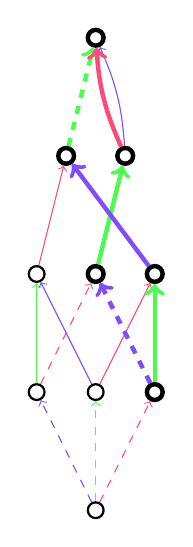
\begin{tikzpicture}[scale=1,bend angle=10]
\newcommand{\xspace}{1}
\newcommand{\yspace}{1}
\tikzstyle{vertex}=[draw,thick,circle,minimum size=2mm,inner sep=0pt]
\tikzstyle{edge}=[->]
\tikzstyle{onesided}=[edge,dashed]
\tikzstyle{bothsided}=[edge]
\tikzstyle{unhighlighted}=[]
\tikzstyle{highlighted}=[ultra thick]
\definecolor{s1color}{RGB}{130,76,253}
\definecolor{s2color}{RGB}{76,253,78}
\definecolor{s3color}{RGB}{253,76,124}
\tikzstyle{s1}=[s1color]
\tikzstyle{s2}=[s2color]
\tikzstyle{s3}=[s3color]
\node[vertex,unhighlighted] (0) at (\xspace*0,\yspace*0) {};
\node[vertex,unhighlighted] (1) at (\xspace*-0.75,\yspace*1.5) {};
\node[vertex,unhighlighted] (2) at (\xspace*0,\yspace*1.5) {};
\node[vertex,highlighted] (3) at (\xspace*0.75,\yspace*1.5) {};
\node[vertex,unhighlighted] (4) at (\xspace*-0.75,\yspace*3) {};
\node[vertex,highlighted] (5) at (\xspace*0,\yspace*3) {};
\node[vertex,highlighted] (6) at (\xspace*0.75,\yspace*3) {};
\node[vertex,highlighted] (7) at (\xspace*-0.375,\yspace*4.5) {};
\node[vertex,highlighted] (8) at (\xspace*0.375,\yspace*4.5) {};
\node[vertex,highlighted] (9) at (\xspace*0,\yspace*6) {};
\draw[s1,onesided,unhighlighted] (0) edge (1);
\draw[s2,onesided,unhighlighted] (0) edge (2);
\draw[s3,onesided,unhighlighted] (0) edge (3);
\draw[s2,bothsided,unhighlighted] (1) edge (4);
\draw[s3,onesided,unhighlighted] (1) edge (5);
\draw[s1,bothsided,unhighlighted] (2) edge (4);
\draw[s3,bothsided,unhighlighted] (2) edge (6);
\draw[s1,onesided,highlighted] (3) edge (5);
\draw[s2,bothsided,highlighted] (3) edge (6);
\draw[s3,bothsided,unhighlighted] (4) edge (7);
\draw[s2,bothsided,highlighted] (5) edge (8);
\draw[s1,bothsided,highlighted] (6) edge (7);
\draw[s2,onesided,highlighted] (7) edge (9);
\draw[s1,bothsided,unhighlighted,bend right] (8) edge (9);
\draw[s3,bothsided,highlighted,bend left] (8) edge (9);
\end{tikzpicture}
		\label{fig:wk-prefix-counterexample}
		\caption{Hasse diagram for \ref{exam:wk-prefix-hypothesis}}
	\end{figure}
\end{exam}

\begin{exam}
	\typedlabel{exam:cap-of-three-residuums}
	Let $w \in \ti{\theta}$ and $S_1,S_2,S_3 \subseteq S$. Then $wC_{S_1} \cap wC_{S_2} \cap wC_{S_3} = wC_{S_1 \cap S_2 \cap S_3}$ is not true in general.

	\begin{proof}
		\todo
	\end{proof}
\end{exam}


% \begin{prop}
% 	\typedlabel{prop:counterexample-simplification}
% 	Let $(W,S)$ be a Coxeter system and $K,T,S_1,S_2,S_3$ be like in \ref{ques:main}. Suppose we have $w \in W$ and $a_1,\ldots,a_n \in T \cup S_1$, $b_1,\ldots,b_n \in T \cup S_2$, $c_1,\ldots,c_n \in T \cup S_3$ with
% 	\begin{align*}
% 	w & = w_K \ul a_1 \ldots \ul a_n \\
% 	  & = w_K \ul b_1 \ldots \ul b_n \\
% 	  & = w_K \ul c_1 \ldots \ul c_n
% 	\end{align*}
% 	and \eqref{eq:main} does not hold for these three expressions, i.e. $w \notin w_K C_T$. Then there exist $t_1,\ldots,t_m \in T$ and $a'_1,\ldots,a'_{n-m} \in T \cup S_1$, $b'_1,\ldots,b'_{n-m} \in T \cup S_2$, $c'_1,\ldots,c'_{n-m} \in T \cup S_3$ such that
% 	\begin{align*}
% 		w \ul t_1 \ldots \ul t_m & = w_K \ul a'_1 \cdots \ul a'_{n-m} \\
% 								 & = w_K \ul b'_1 \cdots \ul b'_{n-m} \\
% 								 & = w_K \ul c'_1 \cdots \ul c'_{n-m}
% 	\end{align*}
% 	with $a'_{n-m},b'_{n-m},c'_{n-m} \notin T$.

% 	\begin{proof}
% 		Suppose at least one element of $a_n,b_n,c_n$ to be in $T$, for example $a_n \in T$. Then we can apply $\ul a_n$ to all three expressions. Since $\rho (w \ul a_n) < \rho(w)$ the \ref{prop:exchanged-property-for-twisted-expressions} yields
% 		\begin{align*}
% 			w \ul a_n & = w_K \ul a_1 \ldots \ul a_n \ul a_n = w_K \ul a_1 \ldots \ul a_{n-1} \\
% 					  & = w_K \ul b_1 \ldots \ul b_n \ul a_n = w_K \ul b_1 \ldots \ul {\hat b}_i \ldots \ul b_n \\
% 					  & = w_K \ul c_1 \ldots \ul c_n \ul a_n = w_K \ul c_1 \ldots \ul {\hat c}_j \ldots \ul c_n
% 		\end{align*}
% 		where $\hat \cdot$ means omission. The omission cannot occur within $w_K$ since all three expressions are still of same twisted length and in the first expression we can see, that $w_K \preceq w \ul a_n$ still holds. This step can be repeated until $w = w_K$ or $a_n,b_n,c_n \notin T$.
% 	\end{proof}
% \end{prop}

% \begin{lemm}
% 	\typedlabel{lemm:counterexample-simplification}
% 	A counterexample to \ref{ques:main} can only exist, if there
% 	is an element $u \in w C_T$ and three distinct generators $s_1,s_2,s_3 \in
% 	D_R(u)$ such that $u \ul s_i \notin w C_T$ for $i=1,2,3$.

% 	\begin{proof}
% 		According to \ref{prop:counterexample-simplification}.
% 	\end{proof}
% \end{lemm}

% Suppose we are in a situation like in \ref{ques:main} with $\rho(w) - \rho(w_K) = n$. If $n = 1$, then \ref{eq:main} holds, since $Wk(\theta)$ cannot contain triple edges. We proceed by induction on $n$. There are three twisted expressions
% \begin{align*}
% 	w & = w_K \ul a_1 \ldots \ul a_n \\
% 	  & = w_K \ul b_1 \ldots \ul b_n \\
% 	  & = w_K \ul c_1 \ldots \ul c_n
% \end{align*}
% with $a_i \in T \cup S_1$, $b_i \in T \cup S_2$ and $c_i \in T \cup S_3$. Since $\rho (w \ul a_n) < \rho(w)$ the \ref{prop:exchanged-property-for-twisted-expressions} yields
% \begin{align*}
% 	w \ul a_n & = w_K \ul a_1 \ldots \ul a_n \ul a_n = w_K \ul a_1 \ldots \ul a_{n-1} \\
% 			  & = w_K \ul b_1 \ldots \ul b_n \ul a_n = w_K \ul b_1 \ldots \ul {\hat b}_i \ldots \ul b_n \\
% 			  & = w_K \ul c_1 \ldots \ul c_n \ul a_n = w_K \ul c_1 \ldots \ul {\hat c}_j \ldots \ul c_n
% \end{align*}
% where $\hat \cdot$ means omission. The omission cannot occur within $w_K$ since all three expressions are still of same twisted length and in the first expression we can see, that $w_K \preceq w \ul a_n$ still holds. It is $\rho(w \ul a_n) - \rho(w_K) = n - 1$, hence by induction hypothesis it is $w \ul a_n \in w_K C_T$. Analogues we get $w \ul b_n, w \ul c_n \in w_K C_T$. If we assume at least one generator of $a_n,b_n,c_n$ to be in $T$, say $a_n \in T$, then $w = w \ul a_n \ul a_n \in w_K C_T$, too. Now suppose $a_n,b_n,c_n \notin T$. Then $a_n,b_n,c_n$ are pairwise different.